\section{\Large Desarrollo}

\begin{enumerate}
    \subsection{Obteniendo los datos.}
    \item Ubicar la Estación Base (Base Station - BS), cuya ubicación es 19.503668573568277, -99.1279845883227. Usando Google Maps o por inspección directa estimar la altura a la que se encuentran colocadas las antenas.
          \begin{figure}[H]
              \centering
              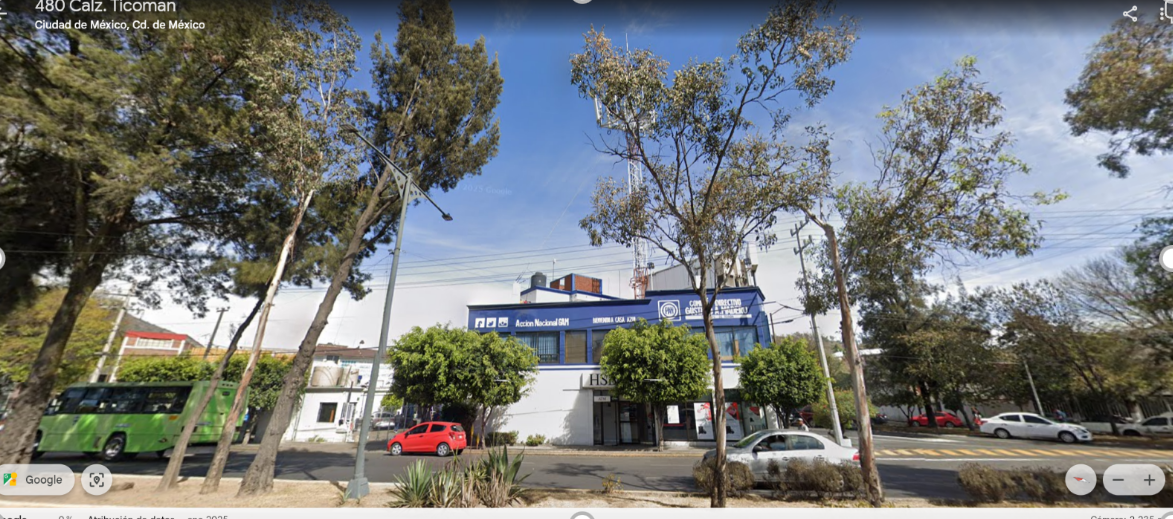
\includegraphics[width=0.9\textwidth]{./img/bs.png}
              \caption{Imagen de la estación base en las coordenadas dadas.}
              \label{fig:bs}
          \end{figure}
    \item Trazar una línea recta entre la BS y la coordenada asignada y calcular la potencia recibida por cada intersección entre una calle y la línea trazada considerando los modelos espacio libre, superficie reflejante, COST231 Walfish-Ikegami y lognormal.
          \textbf{Coordenadas: 19.508953097456004, -99.12414451054960}
          \begin{figure}[H]
              \centering
              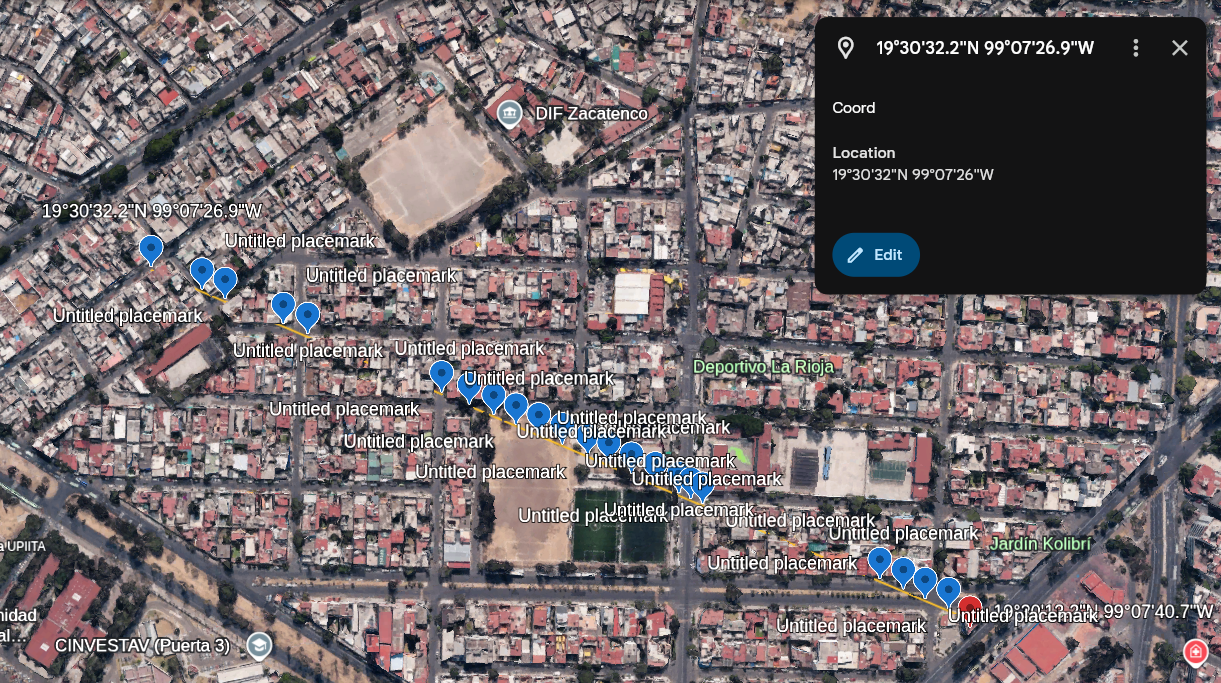
\includegraphics[width=0.9\textwidth]{./img/coordenada-dada.png}
              \caption{Línea recta desde la BS hasta la coordenada asignada.}
              \label{fig:coordenada-dada}
          \end{figure}

          \begin{figure}[H]
              \centering
              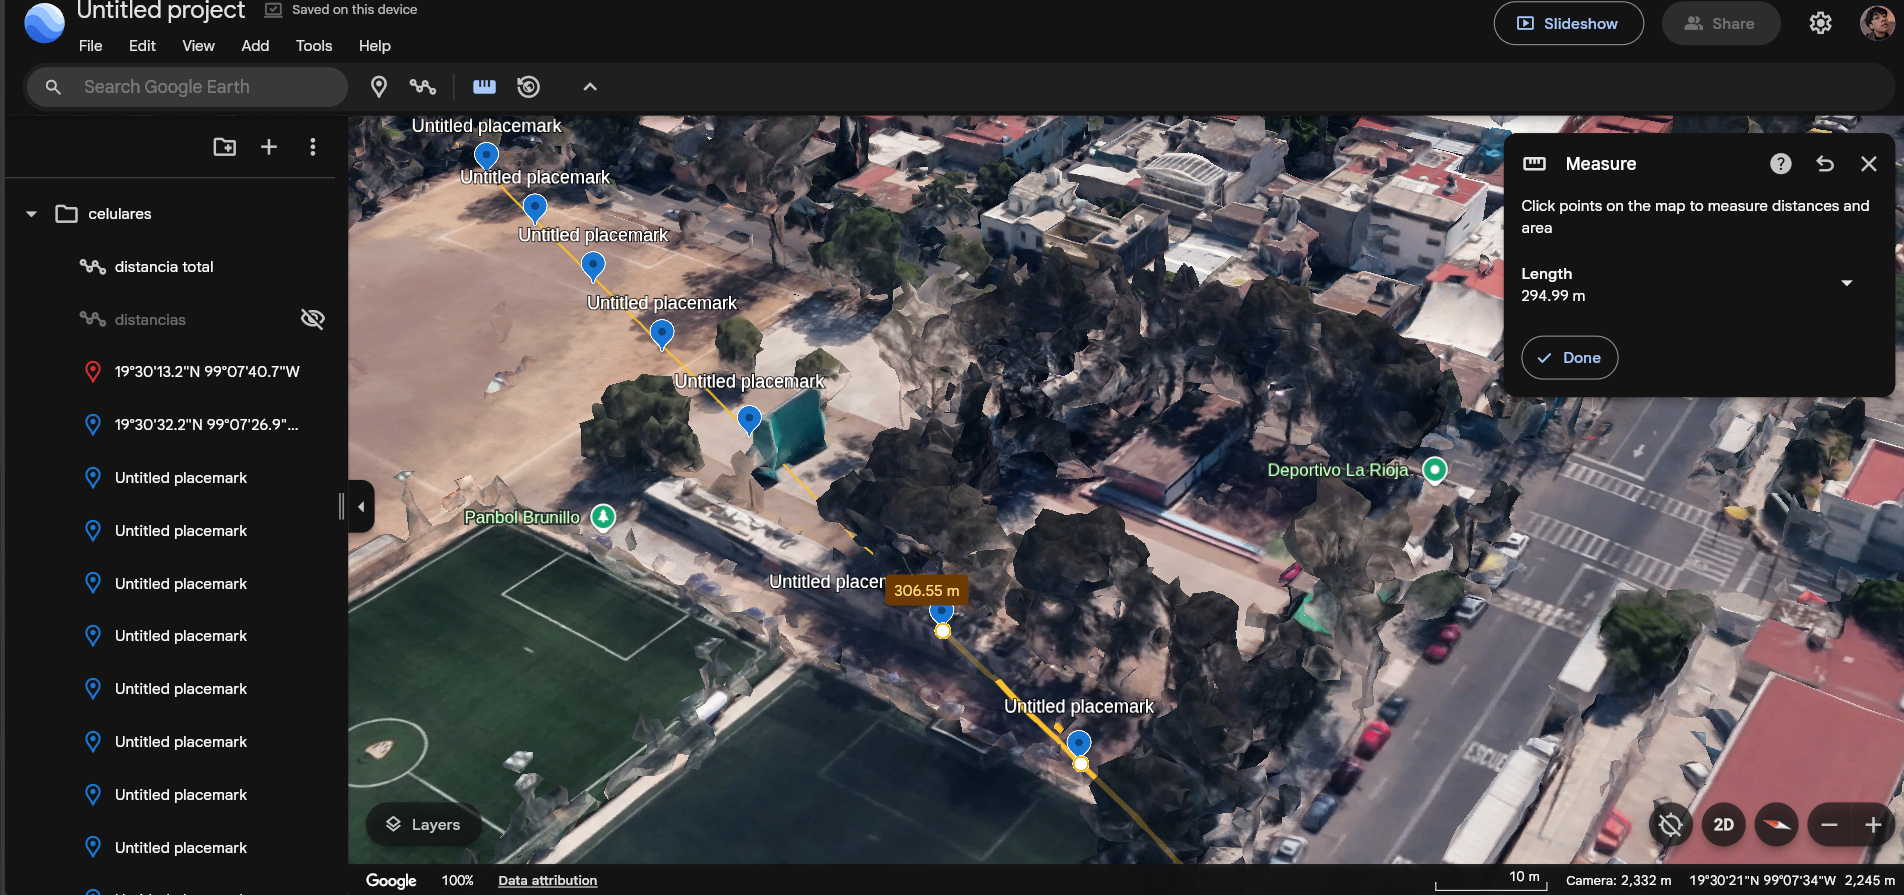
\includegraphics[width=0.9\textwidth]{./img/distancias-puntos.png}
              \caption{Sacando las distancias de la BS a cada punto (aprox cada 20m en exteriores).}
              \label{fig:distancias-puntos}
          \end{figure}
          \begin{figure}[H]
              \centering
              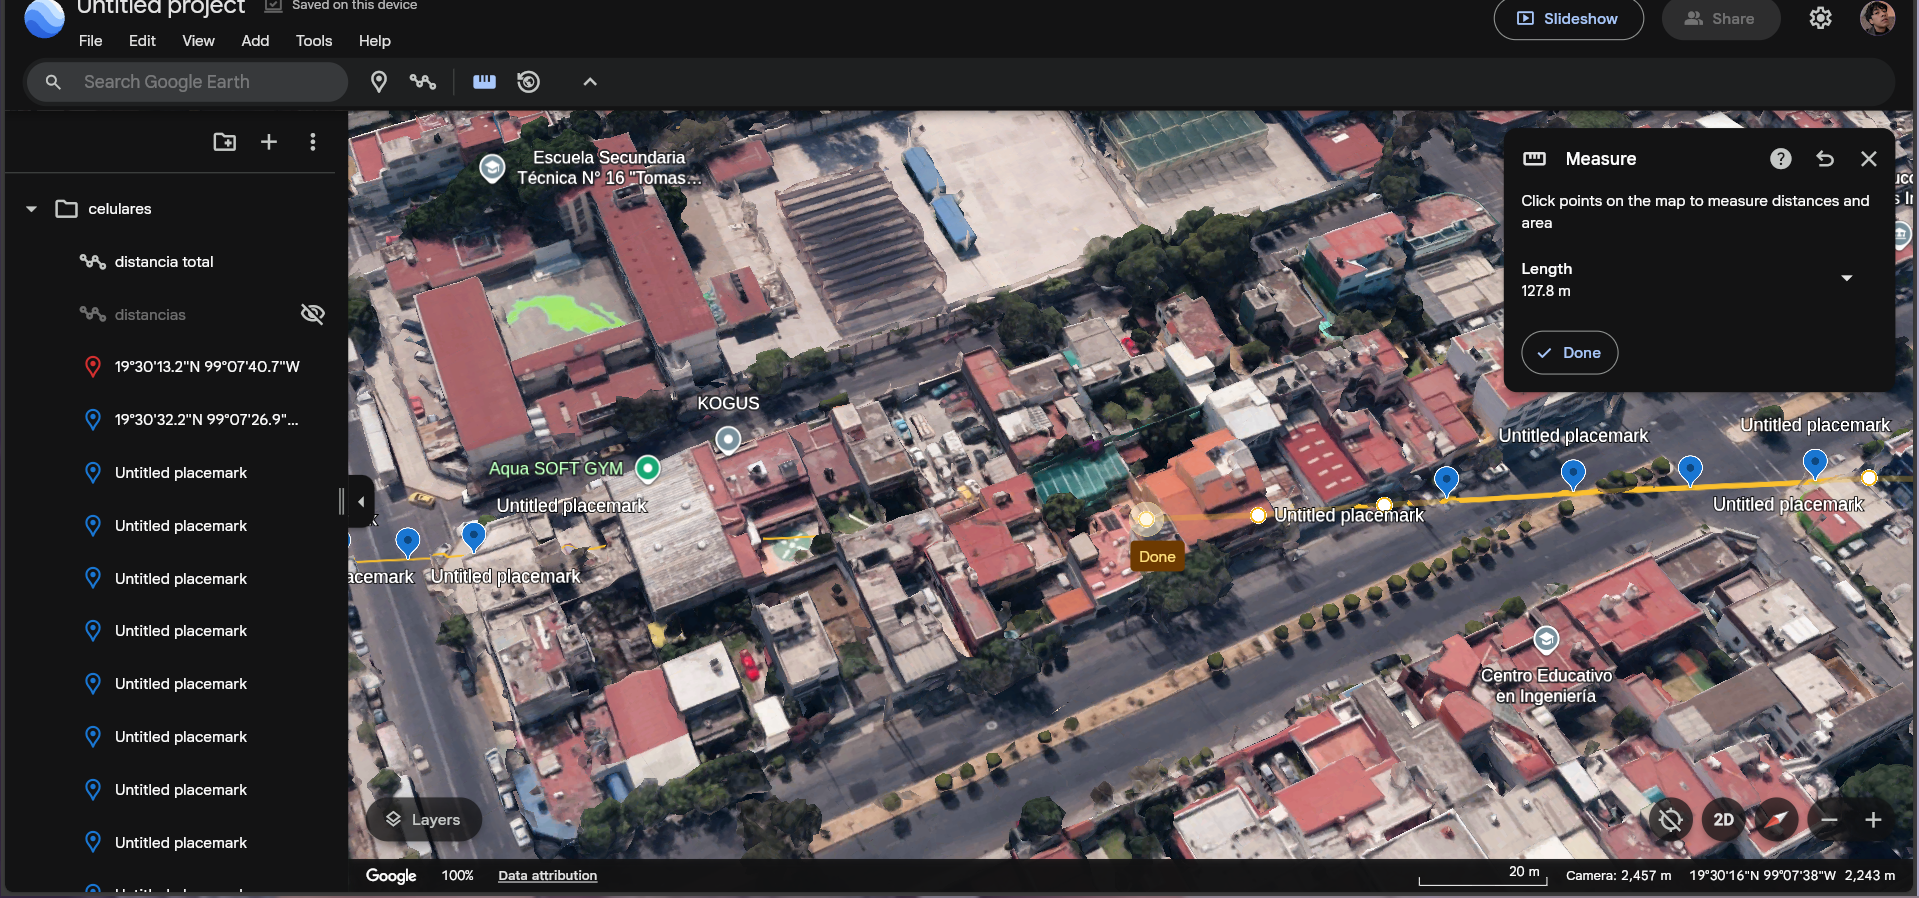
\includegraphics[width=0.9\textwidth]{./img/distancias-edificios.png}
              \caption{Sacando las distancias de los edificios.}
              \label{fig:distancias-edificios}
          \end{figure}
          \begin{figure}[H]
              \centering
              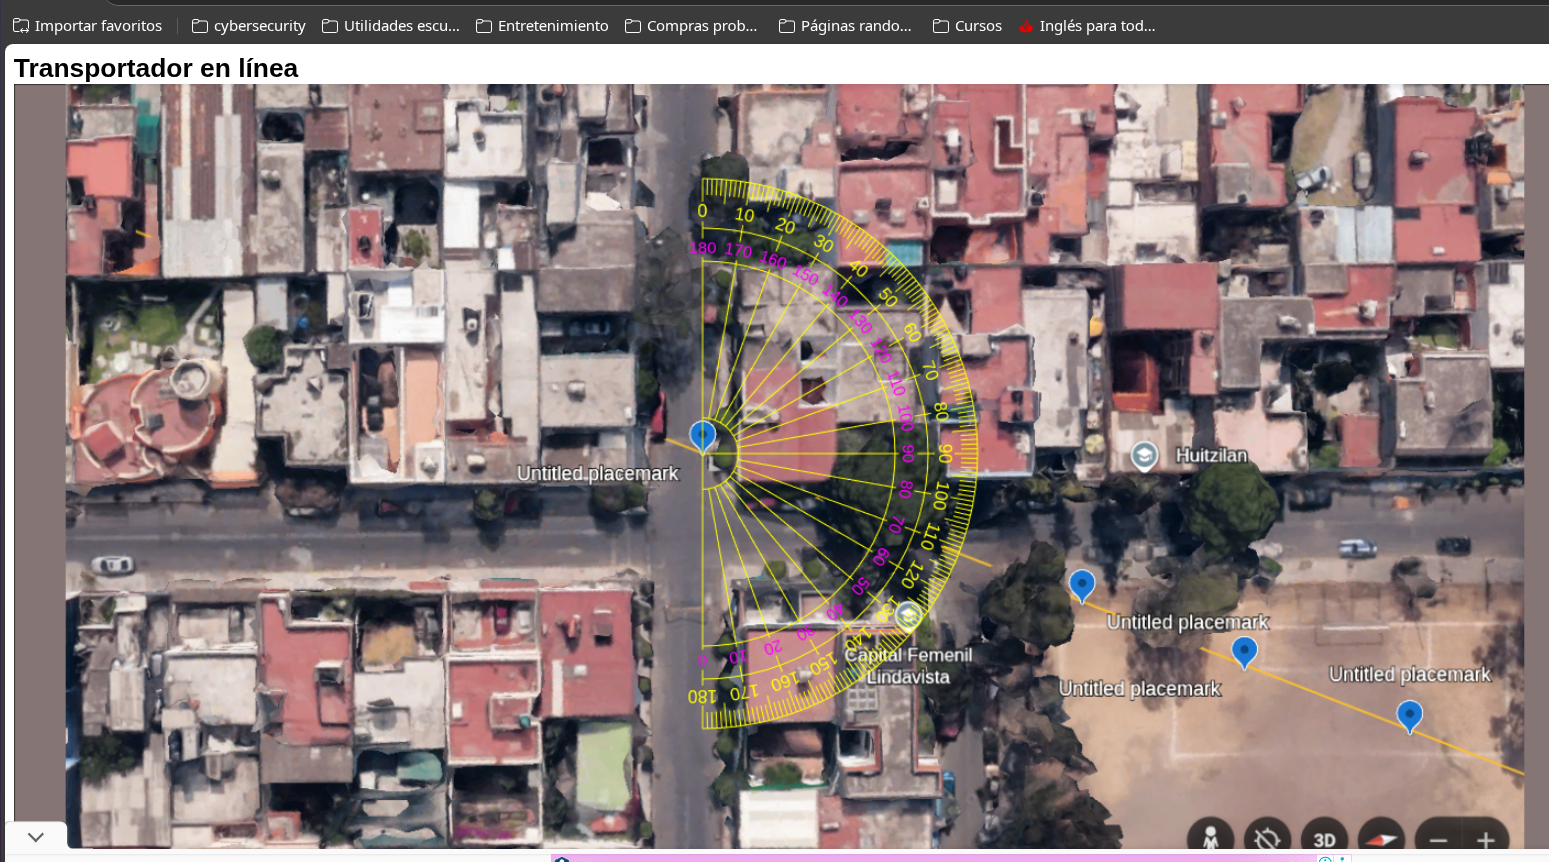
\includegraphics[width=0.9\textwidth]{./img/angulo.png} 
              \caption{Sacando el ángulo de orientación.}
              \label{fig:angulo-orientacion}
          \end{figure}


		  \begin{table}[H]
\centering
\caption{Resultados del Modelo de Espacio Libre}
\label{tab:espacio_libre}
\resizebox{\textwidth}{!}{%
\begin{tabular}{|c|c|c|c|c|}
\hline
\textbf{Punto} & \textbf{Distancia (m)} & \textbf{Pérdidas FSPL (dB)} & \textbf{$P_{rx}$ (dBm)} & \textbf{Coordenadas} \\
\hline
1 & 31.12 & 68.04 & -16.04 & 19.5037, -99.1280 \\
\hline
2 & 47.42 & 71.69 & -19.69 & 19.5038, -99.1279 \\
\hline
3 & 64.68 & 74.39 & -22.39 & 19.5039, -99.1278 \\
\hline
4 & 83.99 & 76.66 & -24.66 & 19.5040, -99.1277 \\
\hline
5 & 234.69 & 85.58 & -33.58 & 19.5045, -99.1272 \\
\hline
6 & 255.27 & 86.31 & -34.31 & 19.5046, -99.1271 \\
\hline
7 & 275.42 & 86.97 & -34.97 & 19.5047, -99.1270 \\
\hline
8 & 295.88 & 87.60 & -35.60 & 19.5048, -99.1269 \\
\hline
9 & 316.21 & 88.17 & -36.17 & 19.5049, -99.1268 \\
\hline
10 & 334.04 & 88.65 & -36.65 & 19.5050, -99.1267 \\
\hline
11 & 355.48 & 89.19 & -37.19 & 19.5051, -99.1266 \\
\hline
12 & 376.08 & 89.68 & -37.68 & 19.5052, -99.1265 \\
\hline
13 & 395.60 & 90.12 & -38.12 & 19.5053, -99.1264 \\
\hline
14 & 414.84 & 90.53 & -38.53 & 19.5054, -99.1263 \\
\hline
15 & 435.31 & 90.95 & -38.95 & 19.5055, -99.1262 \\
\hline
16 & 459.73 & 91.42 & -39.42 & 19.5056, -99.1261 \\
\hline
17 & 575.98 & 93.38 & -41.38 & 19.5061, -99.1256 \\
\hline
18 & 596.64 & 93.69 & -41.69 & 19.5062, -99.1255 \\
\hline
19 & 646.94 & 94.39 & -42.39 & 19.5067, -99.1250 \\
\hline
20 & 666.43 & 94.65 & -42.65 & 19.5068, -99.1249 \\
\hline
21 & 710.86 & 95.21 & -43.21 & 19.5072, -99.1245 \\
\hline
\end{tabular}%
}
\end{table}

\begin{table}[H]
\centering
\caption{Resultados del Modelo de Superficie Reflejante (Two-Ray)}
\label{tab:superficie_reflejante}
\resizebox{\textwidth}{!}{%
\begin{tabular}{|c|c|c|c|}
\hline
\textbf{Punto} & \textbf{Distancia (m)} & \textbf{$P_{rx}$ (dBm)} & \textbf{Coordenadas} \\
\hline
1 & 31.12 & 39.77 & 19.5037, -99.1280 \\
\hline
2 & 47.42 & 32.46 & 19.5038, -99.1279 \\
\hline
3 & 64.68 & 27.07 & 19.5039, -99.1278 \\
\hline
4 & 83.99 & 22.53 & 19.5040, -99.1277 \\
\hline
5 & 234.69 & 4.68 & 19.5045, -99.1272 \\
\hline
6 & 255.27 & 3.22 & 19.5046, -99.1271 \\
\hline
7 & 275.42 & 1.90 & 19.5047, -99.1270 \\
\hline
8 & 295.88 & 0.65 & 19.5048, -99.1269 \\
\hline
9 & 316.21 & -0.50 & 19.5049, -99.1268 \\
\hline
10 & 334.04 & -1.46 & 19.5050, -99.1267 \\
\hline
11 & 355.48 & -2.54 & 19.5051, -99.1266 \\
\hline
12 & 376.08 & -3.52 & 19.5052, -99.1265 \\
\hline
13 & 395.60 & -4.39 & 19.5053, -99.1264 \\
\hline
14 & 414.84 & -5.22 & 19.5054, -99.1263 \\
\hline
15 & 435.31 & -6.06 & 19.5055, -99.1262 \\
\hline
16 & 459.73 & -7.00 & 19.5056, -99.1261 \\
\hline
17 & 575.98 & -10.92 & 19.5061, -99.1256 \\
\hline
18 & 596.64 & -11.53 & 19.5062, -99.1255 \\
\hline
19 & 646.94 & -12.94 & 19.5067, -99.1250 \\
\hline
20 & 666.43 & -13.45 & 19.5068, -99.1249 \\
\hline
21 & 710.86 & -14.58 & 19.5072, -99.1245 \\
\hline
\end{tabular}%
}
\end{table}

    \item Considerar una frecuencia de operación de 1,935 MHz para los modelos que lo requieran. Además, considerar que la potencia de transmisión es de 10W y que las ganancias de las antenas transmisora y receptora son 9 y 3 dB, respectivamente.
    \item Para el modelo COST231 Walfish-Ikegami realizar una tabla con los siguientes datos por cada punto analizado:
          \begin{enumerate}
              \item Coordenadas
              \item Distancia a la EB
              \item Si existe LOS o no
              \item Separación promedio entre edificios, b (si aplica)
              \item Ancho de la "calle" en la que se encuentra el móvil, w (si aplica)
              \item Altura promedio de edificios, h (si aplica)
              \item Ángulo de orientación, $\phi$ (si aplica)
              \item $L_0$
              \item $L_{rts}$ (si aplica)
              \item $L_{msd}$ (si aplica)
              \item Potencia recibida (en dBm)
          \end{enumerate}
          
          \begin{table}[H]
\centering
\caption{Resultados completos del Modelo COST231 Walfish-Ikegami}
\label{tab:walfish_results_complete}
\resizebox{\textwidth}{!}{%
\begin{tabular}{|c|c|c|c|c|c|c|c|c|c|c|}
\hline
\textbf{Pto} & \textbf{Dist (m)} & \textbf{LOS} & \textbf{$\phi$ (°)} & \textbf{b (m)} & \textbf{w (m)} & \textbf{h (m)} & \textbf{$L_0$ (dB)} & \textbf{$L_{rts}$ (dB)} & \textbf{$L_{msd}$ (dB)} & \textbf{$P_{rx}$ (dBm)} \\
\hline
1 & 31.1 & Sí & 22.0 & 59.6 & 30.1 & 7.2 & 69.15 & - & - & -17.15 \\ 
\hline
2 & 47.4 & Sí & 22.0 & 59.6 & 26.4 & 7.2 & 73.91 & - & - & -21.91 \\
\hline
3 & 64.7 & Sí & 22.0 & 59.6 & 26.4 & 7.2 & 77.41 & - & - & -25.41 \\
\hline
4 & 84.0 & Sí & 22.0 & 59.6 & 26.4 & 7.2 & 80.36 & - & - & -28.36 \\
\hline
5 & 234.7 & No & 68.0 & 59.6 & 16.1 & 7.2 & 112.97 & 31.17 & -3.79 & -60.97 \\
\hline
6 & 255.3 & No & 68.0 & 59.6 & 25.1 & 7.2 & 112.42 & 29.24 & -3.13 & -60.42 \\
\hline
7 & 275.4 & No & 21.0 & 59.6 & 8.1 & 7.2 & 113.51 & 29.07 & -2.53 & -61.51 \\
\hline
8 & 295.9 & Sí & 0.0 & 59.6 & 0.0 & 7.2 & 94.58 & - & - & -42.58 \\
\hline
9 & 316.2 & Sí & 0.0 & 59.6 & 0.0 & 7.2 & 95.33 & - & - & -43.33 \\
\hline
10 & 334.0 & Sí & 0.0 & 59.6 & 0.0 & 7.2 & 95.95 & - & - & -43.95 \\
\hline
11 & 355.5 & Sí & 0.0 & 59.6 & 0.0 & 7.2 & 96.65 & - & - & -44.65 \\
\hline
12 & 376.1 & Sí & 0.0 & 59.6 & 0.0 & 7.2 & 97.29 & - & - & -45.29 \\
\hline
13 & 395.6 & Sí & 0.0 & 59.6 & 0.0 & 7.2 & 97.86 & - & - & -45.86 \\
\hline
14 & 414.8 & Sí & 0.0 & 59.6 & 0.0 & 7.2 & 98.40 & - & - & -46.40 \\
\hline
15 & 435.3 & Sí & 23.0 & 59.6 & 11.4 & 7.2 & 98.94 & - & - & -46.94 \\
\hline
16 & 459.7 & No & 23.0 & 59.6 & 9.9 & 7.2 & 121.78 & 28.88 & 1.47 & -69.78 \\
\hline
17 & 576.0 & No & 23.0 & 59.6 & 10.6 & 7.2 & 125.21 & 28.59 & 3.23 & -73.21 \\
\hline
18 & 596.6 & No & 21.0 & 59.6 & 10.6 & 7.2 & 125.08 & 27.89 & 3.51 & -73.08 \\
\hline
19 & 646.9 & No & 55.0 & 59.6 & 10.6 & 7.2 & 133.00 & 34.46 & 4.14 & -81.00 \\
\hline
20 & 666.4 & No & 29.0 & 59.6 & 5.5 & 7.2 & 132.59 & 33.57 & 4.37 & -80.59 \\
\hline
21 & 710.9 & No & 60.0 & 59.6 & 9.7 & 7.2 & 134.38 & 34.30 & 4.88 & -82.38 \\
\hline
\end{tabular}%
}
\end{table}

La determinación de línea de vista (LoS, por sus siglas en inglés) se realizó mediante un análisis trigonométrico. Para cada punto móvil, se trazó una línea recta entre la estación base, ubicada a una altura $h_{\text{bs}}$, y el receptor móvil, a una distancia horizontal $d_{\text{rx}}$ y altura $h_{\text{mvs}}$. La pendiente de esta línea de visión se calcula como:

\[
m = \frac{h_{\text{mvs}} - h_{\text{bs}}}{d_{\text{rx}}}
\]

Luego, para cada edificio situado a una distancia $x$ desde la estación base, se determinó la altura que tendría la línea de visión en dicha posición:

\[
h_{\text{línea}}(x) = h_{\text{bs}} + m \cdot x
\]

    \item Para el modelo lognormal, considere $\alpha$=2.8 y $\sigma$=7dB y realizar una tabla con los siguientes datos por cada punto analizado:
          \begin{enumerate}
              \item Coordenadas
              \item Distancia a la EB
              \item Pérdidas por distancia
              \item Pérdidas por ensombrecimiento
              \item Potencia recibida (en dBm)
          \end{enumerate}
          \begin{table}[H]
\centering
\caption{Resultados del Modelo Lognormal ($\alpha=2.8$, $\sigma=7$ dB)}
\label{tab:lognormal_results}
\resizebox{\textwidth}{!}{%
\begin{tabular}{|c|c|c|c|c|c|}
\hline
\textbf{Punto} & \textbf{Coordenadas} & \textbf{Distancia (m)} & \textbf{Pérdidas (dB)} & \textbf{Ensomb. (dB)} & \textbf{$P_{rx}$ (dBm)} \\
\hline
1 & 19.5037, -99.1280 & 31.12 & -42.19 & 2.46 & 91.73 \\
\hline
2 & 19.5038, -99.1279 & 47.42 & -37.07 & 5.91 & 83.16 \\
\hline
3 & 19.5039, -99.1278 & 64.68 & -33.30 & 1.79 & 83.51 \\
\hline
4 & 19.5040, -99.1277 & 83.99 & -30.12 & 0.12 & 82.00 \\
\hline
5 & 19.5045, -99.1272 & 234.69 & -17.63 & -2.87 & 72.50 \\
\hline
6 & 19.5046, -99.1271 & 255.27 & -16.60 & 2.59 & 66.02 \\
\hline
7 & 19.5047, -99.1270 & 275.42 & -15.68 & 6.75 & 60.93 \\
\hline
8 & 19.5048, -99.1269 & 295.88 & -14.81 & 1.64 & 65.17 \\
\hline
9 & 19.5049, -99.1268 & 316.21 & -14.00 & 1.33 & 64.67 \\
\hline
10 & 19.5050, -99.1267 & 334.04 & -13.33 & -2.19 & 67.53 \\
\hline
11 & 19.5051, -99.1266 & 355.48 & -12.58 & 2.29 & 62.29 \\
\hline
12 & 19.5052, -99.1265 & 376.08 & -11.89 & 9.88 & 54.01 \\
\hline
13 & 19.5053, -99.1264 & 395.60 & -11.28 & -4.54 & 67.82 \\
\hline
14 & 19.5054, -99.1263 & 414.84 & -10.70 & -2.81 & 65.51 \\
\hline
15 & 19.5055, -99.1262 & 435.31 & -10.11 & 3.92 & 58.19 \\
\hline
16 & 19.5056, -99.1261 & 459.73 & -9.45 & -2.41 & 63.86 \\
\hline
17 & 19.5061, -99.1256 & 575.98 & -6.71 & -3.23 & 61.94 \\
\hline
18 & 19.5062, -99.1255 & 596.64 & -6.28 & 1.23 & 57.05 \\
\hline
19 & 19.5067, -99.1250 & 646.94 & -5.30 & -11.87 & 69.16 \\
\hline
20 & 19.5068, -99.1249 & 666.43 & -4.93 & -6.70 & 63.63 \\
\hline
21 & 19.5072, -99.1245 & 710.86 & -4.15 & -9.54 & 65.70 \\
\hline
\end{tabular}%
}
\end{table}
\newpage
    \item Realizar una figura en la que muestre la potencia recibida en función de la distancia para cada uno de los modelos y escribir un análisis de estos resultados

\subsection{Comparación de Modelos de Propagación}

\begin{figure}[H]
    \centering
    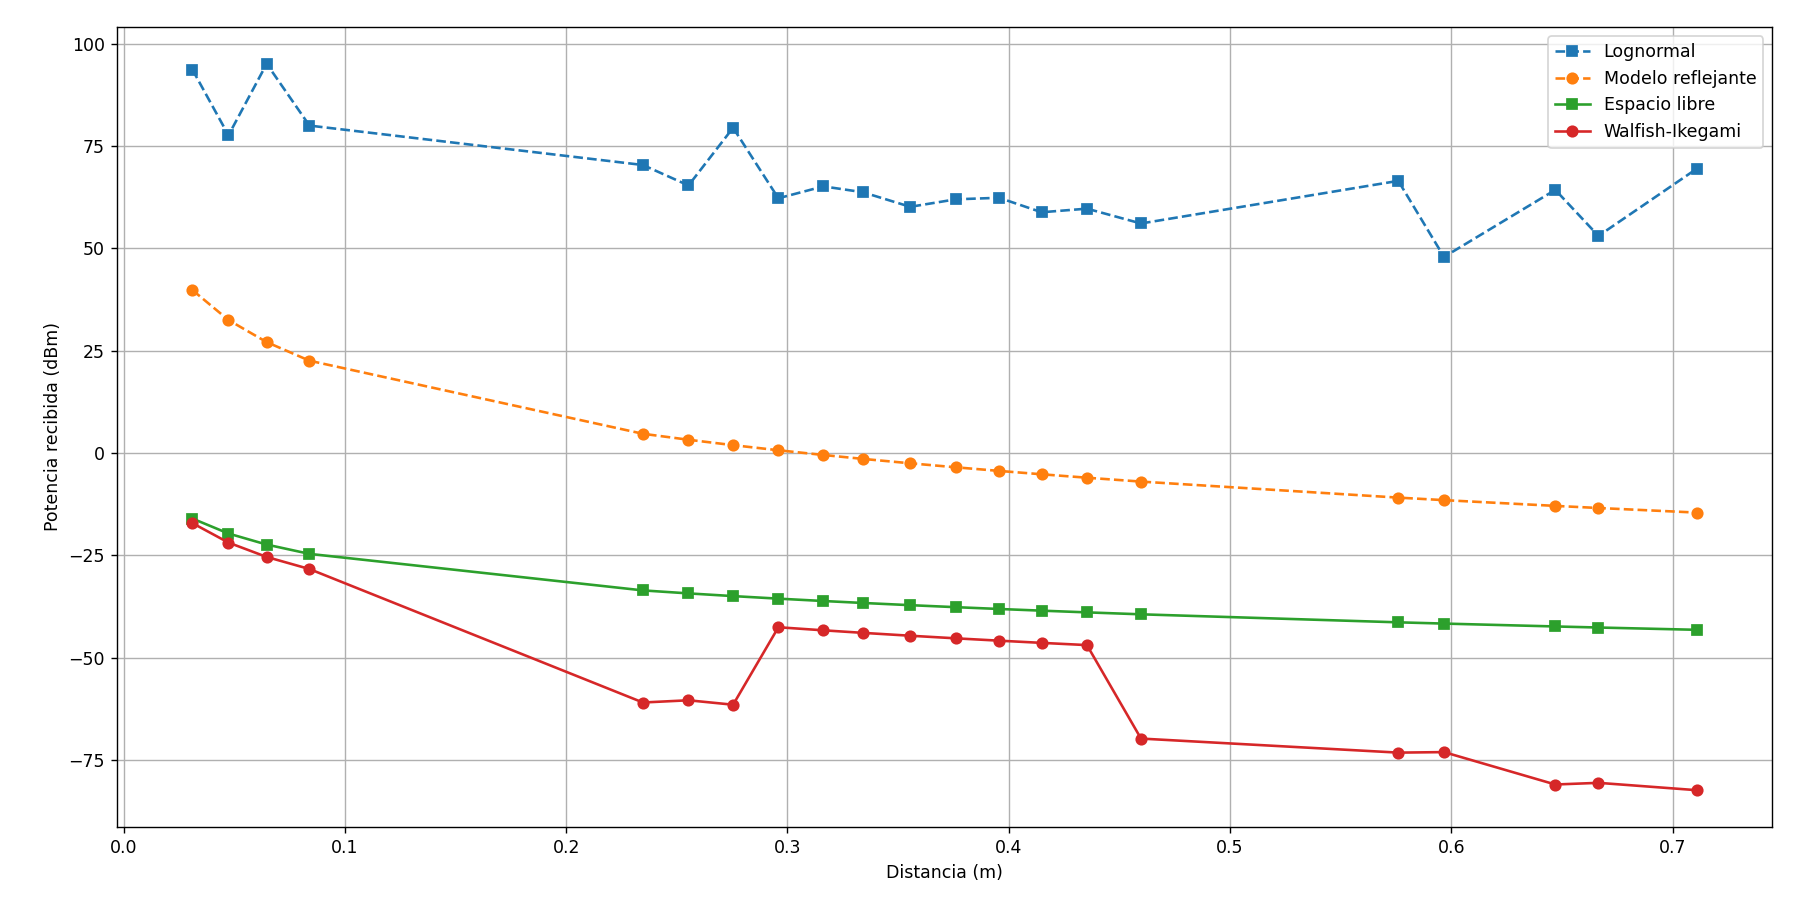
\includegraphics[width=0.9\textwidth]{./img/grafica.png}
    \caption{Comparación de potencia recibida vs distancia para los diferentes modelos de propagación}
    \label{fig:comparacion_modelos}
\end{figure}

\subsection{Análisis comparativo}

Los resultados obtenidos muestran diferencias significativas entre los modelos evaluados:

\begin{itemize}
    \item \textbf{Modelo de Espacio Libre:} Presenta una atenuación constante y gradual, siguiendo el comportamiento teórico esperado $L = 32.44 + 20\log_{10}(d_{km}) + 20\log_{10}(f_{MHz})$.
    
    \item \textbf{Modelo de Superficie Reflejante:} Muestra una caída más pronunciada, especialmente notable en distancias menores a 100 metros, donde el efecto de interferencia entre la onda directa y la reflejada es más significativo.
    
    \item \textbf{Modelo COST231 Walfish-Ikegami:} Presenta un comportamiento intermedio con variaciones abruptas en los puntos NLOS (Non-Line-of-Sight), donde las pérdidas adicionales ($L_{rts}$) y ($L_{msd}$) son consideradas. 
    
    \item \textbf{Modelo Lognormal:} Exhibe la mayor variabilidad debido al componente de desvanecimiento por sombra ($\sigma=7$ dB). La potencia recibida sigue la expresión:
    \begin{equation}
        P_r = P_t + G_t + G_r - (10\alpha\log_{10}(d) + X_\sigma)
    \end{equation}
    donde $X_\sigma$ es la variable aleatoria gaussiana con $\sigma=7$ dB.
\end{itemize}

\begin{itemize}
    \item El modelo \textbf{Superficie-Reflejante} predice mayores niveles de potencia en distancias cortas ($<$150 m) pero una atenuación más rápida que el espacio libre en distancias mayores, debido al efecto de interferencia destructiva.
    
    \item El modelo \textbf{Walfish-Ikegami} es el más adecuado para entornos urbanos, mostrando cómo la presencia de edificios (altura promedio $h=7.23$ m) afecta significativamente la propagación, con diferencias de hasta 20 dB entre puntos LOS y NLOS.
    
    \item La variabilidad del modelo \textbf{Lognormal} ($\sigma=7$ dB) resalta la importancia de considerar márgenes de desvanecimiento en el diseño del sistema. Por ejemplo, para garantizar una probabilidad del 90\% de cobertura, se requeriría un margen adicional de aproximadamente 9 dB.
    
\end{itemize}

\end{enumerate}